\documentclass[../main.tex]{subfiles}
\begin{document}

\chapter{Certificazione e accreditamento}
Questo capitolo affronterà la certificazione di sicurezza in ambito di \textit{web-services}, illustrando i criteri, le metodologie e i paradigmi implicati.
Per "\textit{certificazione}" si intende l'insieme di procedure impiegate nel processo di erogazione di un certificato, ovvero la produzione di un documento attestante la compatibilità tra le caratteristiche di un sistema o di una procedura e i requisiti prestabiliti da una norma o da uno standard.
L'"\textit{accreditamento}" è invece la dichiarazione formale da parte di una terza parte fidata che il processo di certificazione sia a sua volta compatibile con uno standard riconosciuto.
In ambito di sicurezza informatica, certificazione e accreditamento possono essere intesi come parti di un unico processo: \textit{Certification and Accreditation (C\&A)} \cite{NistCAHandbook}.

La fase di certificazione comprende un'analisi del sistema per identificare le possibili debolezze e le relative contromisure in un particolare ambiente e un'analisi delle potenziali vulnerabilità causate dalle debolezze individuate \cite{NistCAHandbook}.
La fase di accreditamento rappresenta invece la dichiarazione formale da parte di una "autorità designata all'approvazione" (\textit{Designated Approving Authority, DAA}) che un sistema informatico  automatizzato \textit{(Automated Information System, AIS)} operi in una determinata modalità di sicurezza utilizzando un insieme predefinito di protezioni basato sul rischio residuo identificato durante il processo di certificazione \cite{NistCAHandbook}.

L'accreditatore ha quindi la responsabilità formale di autorizzare l'operatività del sistema e deve rimanere impegnato attivamente nel processo di riaccreditazione durante il ciclo di vita di un sistema, poiché il livello di rischio può cambiare \cite{NistCAHandbook}.
Il processo di accreditazione deve essere implementato all'inizio del ciclo di vita del sistema, per garantire
\begin{itemize}
\item che siano progettati e integrati i meccanismi di sicurezza e le protezioni opportune
\item che le decisioni di sicurezza non vengano ritardate causando costi aggiuntivi
\end{itemize}


\section{Valutazione del software sicuro basata sui \textit{Common Criteria}}
Tradizionalmente, le tecniche di certificazione rappresentano la soluzione di analisi scelta per fornire la prova che un software abbia le proprietà non funzionali desiderate e si comporti come atteso.
Sono state proposte molte soluzione e schemi, alcuni di essi si sono concentrati sulla certificazione delle proprietà di sicurezza del software \cite{CitCertSoa}.
Il primo tentativo in questa direzione risale al 1985, con la creazione dello standard TCSEC, comunemente chiamato "\textit{Orange Book}" \cite{OrangeBook}.
Successivamente sono stati proposti altri standard, come il Common Criteria (CC) del Dicembre 1999, (ISO15408) che rappresenta il punto di riferimento internazionale per la certificazione del software sicuro \cite{HerrmannCC}.
%http://www.sans.org/reading-room/whitepapers/country/applying-common-criteria-certification-accreditation-department-defense-unclass-1171
Esso infatti definisce i concetti generali e i principi della sicurezza informatica, identifica i requisiti di sicurezza per i prodotti e per i sistemi IT e presenta un modello di valutazione basato sui requisiti funzionali - che rappresentano il comportamento desiderato per un prodotto o sistema - e i requisiti di sicurezza, i quali stabiliscono con un certo livello di confidenza che le misure di sicurezza siano implementate nel modo giusto ed effettivamente utilizzate \cite{CommonCriteriaSans}.

\subsection{Organizzazione dei Common Criteria}
L'organizzazione dei Common Criteria introduce una grande flessibilità nella specifica dei prodotti sicuri: grazie ad essi i consumatori possono specificare le funzionalità di sicurezza di un prodotto in termini di \textit{profili di protezione} standardizzati e possono scegliere livelli di \textit{assurance} differenziati per la valutazione di ciascun profilo di protezione (\textit{Evaluation Assurance Level}), da EAL1 a EAL7 \cite{SyntegraCC}.
I \textit{Common Criteria} sono divisi in tre sezioni \cite{CommonCriteriaSans}:
\begin{enumerate}
\item \textit{Introduzione e modello generale}, definisce i termini e i concetti utilizzati durante il processo di valutazione.
\item \textit{Descrizione delle componenti funzionali per la sicurezza} che definiscono i requisiti di sicurezza di un sistema o prodotto IT
\item \textit{Descrizione delle componenti di \textit{assurance}} che vengono utilizzate per misurare l'efficacia dei controlli di sicurezza implementati.
\end{enumerate}.
Ognuna di queste sezioni prevede la collaborazione di tre diversi ruoli:
\begin{itemize}
\item \textit{Consumatori}, che utilizzano il prodotto software o sistema informatico e hanno necessità di sicurezza. Lungo il ciclo di vita del processo di certificazione e accreditamento hanno principalmente un ruolo di riferimento per:
\begin{itemize}
\item Ottenere informazioni di background sullo specifico caso d'uso di un prodotto
\item Formulare le asserzioni per le funzionalità di sicurezza
\item Determinare il corretto livello di \textit{assurance}.
\end{itemize}
\item \textit{Sviluppatori}, che implementano il prodotto software o sistema informatico e le funzionalità di sicurezza. Il loro ruolo è quello di:
\begin{itemize}
\item Fornire informazioni per lo sviluppo dei requisiti di sicurezza e formulare le specifiche per l'identificazione dei \textit{Target of Evaluation (TOE)}
\item Essere un punto di riferimento nell'interpretazione delle asserzioni di sicurezza, per formalizzare correttamente le specifiche funzonali dei \textit{TOE}
\item Essere un punto di riferimento nell'interpretazione delle asserzioni dei requisiti di \textit{assurance} e per determinare gli approcci di \textit{assurance} per i \textit{TOE}
\end{itemize}
\item \textit{Valutatori}, che effettuano la valutazione formale e funzionale del prodotto software o sistema informatico. Si occupano di:
\begin{itemize}
\item Fornire le informazioni e le istruzioni per la strutturazione dei profili di protezione
\item Determinare se un \textit{TOE} rispetti le funzionalità di sicurezza dichiarate
\item Determinare il livello di assurance di un \textit{TOE} in relazione ai profili di protezione
\end{itemize}
\end{itemize}


I Common Criteria sono organizzati su un albero a tre livelli, come mostrato in figura \ref{fig:FigCCStruct}.
\begin{figure}[H]
   \centering
   \makebox[\textwidth]{
   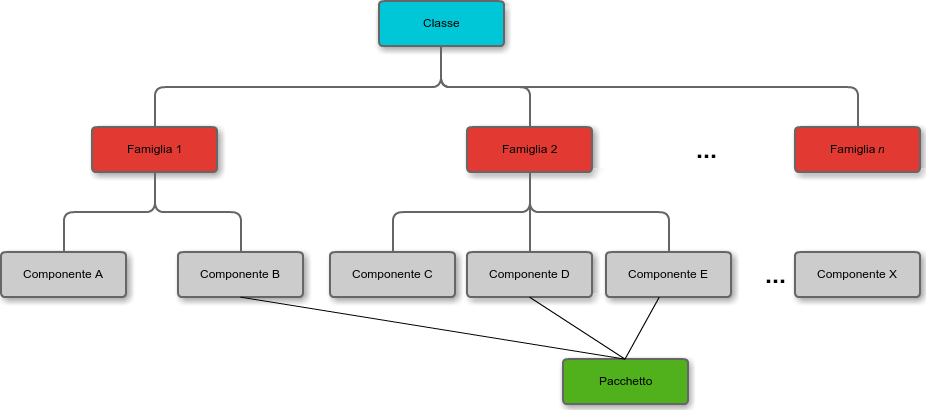
\includegraphics[width=\textwidth]{immagini/CommonCriteria.png}
   }
   \caption{Struttura Common Criteria \cite{SyntegraCC}}\label{fig:FigCCStruct}
\end{figure}.
I livelli possono essere così descritti:
\begin{itemize}
\item \textbf{Classi}: raggruppamenti di funzionalità di sicurezza in base a requisiti funzionali comuni (es. \textit{autenticazione}, \textit{gestione della sicurezza}, \textit{protezione dei dati}, \textit{ sicurezza delle comunicazioni}, \textit{auditing})
\item \textbf{Famiglie} di requisiti di sicurezza: ogni \textit{classe} contiene delle \textit{famiglie} di requisiti di sicurezza che corrispondono a uno specifico obiettivo da raggiungere.
\item \textbf{Componenti}: ogni famiglia comprende dei componenti, che rappresentano la specifica istanza e le procedure specifiche che devono essere eseguite per il raggiungimento dell'obiettivo.
\end{itemize}
Infine, la combinazione tra un sottoinsieme di requisiti e di un sottoinsieme di obiettivi di sicurezza, è chiamata \textbf{Pacchetto}.

\subsection{Usare i Common Criteria nel processo di certificazione e accreditamento}
Il processo di certificazione e accreditamento prevede il coinvolgimento di tre diverse tipologie di attori - alle quali corrispondono altrettante fasi - ognuna delle quali ha determinate responsabilità:
\begin{itemize}
\item \textbf{Sviluppatori del sistema}, a supporto della comunità degli utenti.\newline
\item \textbf{Valutatori del sistema}, a supporto della Certification Authority
\item \textbf{Accreditatori individuali}
\end{itemize}

\subsubsection{Fase di sviluppo del sistema}
Possono utilizzare i Common Criteria per la progettazione del sistema, sfruttando i \textit{Protection Profiles} per identificare le proprietà da rispettare per garantire la conformità con i requisiti di sicurezza.
Un \textit{Protection Profile} descrive un insieme di requisiti e obiettivi di sicurezza indipendenti dall''implementazione, in relazione alle vulnerabilità presenti nell'ambiente specificato. Ciò consente inoltre l'interazione tra la community degli utenti e gli sviluppatori, per creare un insieme di requisiti di sicurezza riutilizzabile e standardizzato \cite{CommonCriteriaSans}.
Esso può essere usato quando:
\begin{itemize}
\item un gruppo di utenti necessita di requisiti di sicurezza per una determinata applicazione del prodotto
\item un ente governativo necessita di requisiti di sicurezza per una classe di prodotti (es. firewall)
\item un'organizzazione vuole comprare un sistema certificato per la gestione dei suoi specifici requisiti di sicurezza (es. registrazione dei pazienti in un ospedale)
\end{itemize}
Nella definizione dei requisiti di sicurezza, gli sviluppatori devono anche considerare le minacce all'ambiente operativo. A tal fine i Common Criteria contengono un catalogo di componenti da cui gli sviluppatori dei \textit{profili di protezione} possono attingere. Il profilo di protezione è organizzato secondo una struttura gerarchica, così da permettere di individuare con facilità il componente adatto alla risoluzione di una specifica problematica di sicurezza.
Al fine di documentare la compatibilità tra un sistema informatico con i requisiti derivati dai \textit{profili di protezione}, deve essere sviluppato un \textit{System Security Authorization Agreement}. Esso ha il fine di fornire una descrizione completa del sistema, di come la sicurezza è stata implementata e del contesto in cui sono stati progettati, sviluppati ed eseguiti i test e le procedure di valutazione \cite{CommonCriteriaSans}.
Per esempio, se il sistema fornisce un metodo per l'autenticazione e l'identificazione dell'utente, il \textit{SSAA} deve documentarne il funzionamento; se ci sono dei requisiti per effettuare l'auditing di determinati eventi, devono essere descritti.
Inoltre è necessario includere tutte le assunzioni fatte a proposito dell'ambiente, specificando tutti i controlli di sicurezza fatti nei confronti della struttura fisica dello stesso, del personale e della connetttività.
Esso è dunque un \textit{living document}: è di fondamentale importanza che venga aggiornato in base a decisioni successive e alle eventuali discrepanze identificate durante la fase di testing e valutazione.


\subsection{Fase di valutazione del sistema}
Durante questa fase i valutatori (generalmente assegnati dalla \textit{Certification Authority}) eseguono una revisione del sistema per determinare se ciascuna delle vulnerabilità identificate durante lo sviluppo dei \textit{Protection Profile} siano state gestite e/o mitigate in modo opportuno.
Viene quindi introdotto il \textit{TOE} (\textit{Target of Evaluation}), che rappresenta il prodotto o sistema informatico oggetto della valutazione, unito alla relativa documentazione e alle configurazioni dell'ambiente in cui opera e della rete.
Gli obiettivi e i requisiti di sicurezza per uno specifico \textit{TOE} sono specificati nel \textit{ST} (\textit{Security Target}), il quale ha il compito di descrivere nel dettaglio le misure di sicurezza implementate e di garantirne la compatibilità con i requisiti stessi.
Un \textit{ST} può essere conforme a uno o più \textit{profili di protezione} e costituisce quindi la base del processo di valutazione della sicurezza di un sistema informatico.
I valutatori hanno quindi il compito di verificare che sia stato raggiunto un livello di sicurezza adeguato e che le procedure di installazione, configurazione e avvio di un prodotto siano state effettuate in maniera idonea a quanto espresso nel \textit{Security Target}.
Il risultato atteso del processo di valutazione è la conferma che un \textit{ST} è soddisfatto per un determinato \textit{TOE}, unito a un report che documenti in modo dettagliato tutto il processo.

\subsection{Fase di testing del sistema}
L'attività più corposa e complessa del processo di certificazione e accreditamento è lo sviluppo - effettuato mediante l'utilizzo dei requisiti funzionali e di assurance descritti dai \textit{Common Criteria} - e l'esecuzione delle procedure di test atte a verificare l'effettiva compatibilità del sistema con i requisiti di sicurezza precedentemente definiti.
Affinché possa essere garantita l'efficienza del testing, è necessario che il \textit{System Security Authorization Agreement} fornisca una base adeguata per il sviluppo delle procedure di test e di valutazione.

Dopo il completamento della fase di testing, viene redatto un report formale dei risultati, comprendente tutte le discrepanze identificate.
Le eventuali problematiche vengono quindi corrette e viene nuovamente eseguita la fase di testing. Nel caso in cui la correzione non sia possibile oppure la soluzione sia troppo costosa, esse vengono tralasciate e trattate come \textit{rischi residui}.
La Certification Authority presenterà quindi all'accreditatore un pacchetto di certificazione composto dall'\textit{SSAA} e da tutta la documentazione di supporto, i risultati della fase di testing e da una lista di tutti i rischi residui del sistema informatico. 
\subsection{Accreditamento e post-accreditamento del sistema}
I Common Criteria sono utili anche agli accreditatori di un sistema, poiché, per stabilire se le proprietà di sicurezza siano rispettare e se il sistema possa operare a un livello di rischio accettabile, è utile avere un punto di riferimento solido per classificare i requisiti funzionali e di assurance.
Se il risultato dell'accreditamento è positivo, il sistema otterrà il certificato di accreditamento (\textit{Authority to Operate}). Al contrario, se i requisiti non sono soddisfatti, verrà emesso un \textit{Interim Authority to Operate} con validità limitata, nel cui periodo di riferimento devono essere risolte tutte le discrepanze individuate.
L'accreditamento è una procedura continuativa nel ciclo di vita di un prodotto. Occorre quindi effettuare attività di monitoraggio e varie operazioni per assicurarsi che il sistema preservi un livello di rischio accettabile. Ogni qualvolta emergono difetti o vulnerabilità, occorre effettuare una nuova valutazione del sistema modificando in modo opportuno il \textit{SSAA}.

\section{Certificazione dei servizi SOA basata sul testing}
%integrare Security Certification of Composite Services: A Test-Based Approach
Le tecniche di certificazione possono giocare un ruolo molto importante anche nell'ecosistema dei servizi, tuttavia le modalità esistenti non si adattano bene a questo scenario. Un ecosistema basato sui servizi è, per definizione, di natura dinamica; le tecniche di certificazione usuali, invece, considerano il software come entità statica e monolitica, fornendo un certificato non formalizzato e utilizzabile solo nella fase di installazione del prodotto.
Abbiamo dunque bisogno di una soluzione che possa essere integrabile nella composizione dei processi di business \cite{DamianiCitCertSoa} \cite{CitCertSoa}.

Un approccio potenzialmente in grado di garantire le esigenze di certificazione per i servizi web, è stato definito nell'articolo \textit{A Test-Based Security Certification Scheme for Web Services} di \textit{Anisetti, M. , Ardagna, C. , Damiani E. e Saonara F.} \cite{CitCertSoa} e si basa su un modello fondato sul testing per fornire le prove che il servizio da certificare rispetti un insieme di proprietà di sicurezza date.
Lo schema di certificazione si basa su casi di test generati automaticamente, in modo da produrre evidenze \textit{machine-readable} per comprovare le proprietà di sicurezza del servizio \cite{CitCertSoa}.

\subsection{Processo di certificazione}


L'obiettivo della certificazione è rappresentato dalla proprietà di sicurezza da certificare.
Il processo descritto è fondato sulla certificazione delle proprietà di sicurezza (confidenzialità, integrità, autenticità) e ha inizio da un \textit{service model} che contiene tutte le informazioni di interesse per effettuare il processo di certificazione.
A partire da esso si producono le evidenze a sostegno della proprietà da certificare.
Alla conclusione del processo, si può affermare che una data proprietà di sicurezza è certificata in base a un determinato \textit{service-model} (Figura \ref{fig:CertSoaFig1a}).

\begin{figure}[H]
\centering
\makebox[\textwidth]{
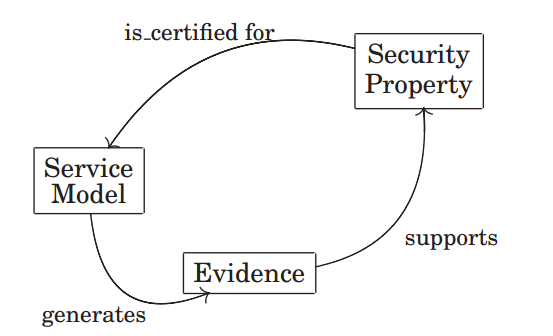
\includegraphics[width=8cm]{immagini/CertSoaFig1a.png}
}
\caption{Fasi del processo di certificazione \cite{CitCertSoa}}\label{fig:CertSoaFig1a}
\end{figure}

Il processo  e viene condotto grazie alla collaborazione di tre attori, la cui interazione è descritta nella figura \ref{fig:CertSoaFig1b}:
\begin{enumerate}
\item Un fornitore di servizi, che necessita della certificazione. Implementa il proprio servizio web e produce:
\begin{itemize}
\item il documento di descrizione delle operazioni in "\textit{Web Service Description Language (WSDL)}".
\item il documento di descrizione delle interfacce e di conversazione con i client in "\textit{Web Service Communication Language (WSCL)}".
\end{itemize}
Dopodiché avvia il processo di certificazione, fornendo all'autorità di certificazione i documenti WSDL e WSCL, l'implementazione del servizio e la lista delle proprietà da certificare. 
\item Un'autorità di certificazione (\textit{certification authority}) che gestisce tutto il processo di certificazione. Una volta ricevute le informazioni dal fornitore di servizi, genera il \textit{service model} e lo invia a un laboratorio accreditato insieme all'implementazione del servizio e alla lista delle proprietà di certificare, fornite al punto 1.
\item Un laboratorio accreditato (\textit{accredited lab}) controllato dall'autorità di certificazione, che  effettua la valutazione delle proprietà. Una volta ricevute le informazioni dalla \textit{certification authority}, effettua la fase di generazione delle evidenze e le restituisce alla stessa. Se queste sono sufficienti, la \textit{certification authority} rilascia un certificato per il servizio, includendo proprietà certificate, il \textit{service model} e le evidenze.
\end{enumerate}

\begin{figure}[H]
\centering
\makebox[\textwidth]{
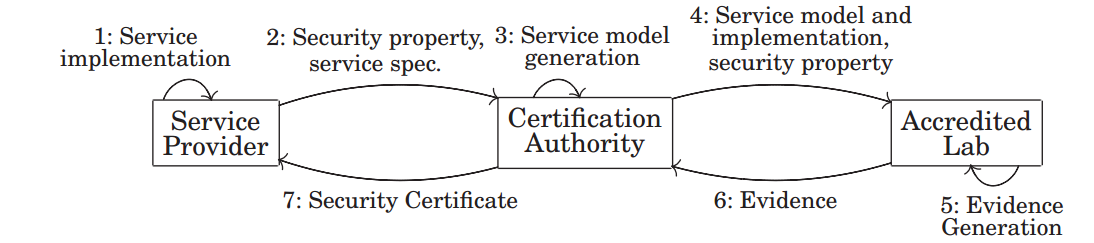
\includegraphics[width=\textwidth]{immagini/CertSoaFig1b.png}
}
\caption{Fasi del processo di certificazione \cite{CitCertSoa}}\label{fig:CertSoaFig1b}
\end{figure}

\section{Certificazione incrementale} %A Low-Cost Security Certification Scheme for Evolving Services
I servizi SOA subiscono nel tempo continui e veloci cambiamenti. Devono perciò essere adattati a nuovi contesti, ad evoluzioni nei processi di business, cambiamenti legali o errori nella definizione stessa del servizio \cite{Casati}.
L'obiettivo delle certificazione incrementale è quello di rinnovare il certificato relativo a un servizio riutilizzando, il più possibile, le evidenze collezionate per l'emissione dei vecchi certificati.
Un processo di questo tipo dovrebbe ridurre i costi e l'\textit{overhead} della certificazione dei servizi in evoluzione \cite{CertEvolutiva}.
Alcuni approcci, per come descritti dal documento, possono essere:
\begin{itemize}
\item \textit{Adattamento della certificazione}: nessuna necessità di effettuare una nuova certificazione. L'aggiornamento può essere effettuato nel momento in cui viene rilasciata una nuova versione del \textit{service-model}, senza richiedere la generazione e l'esecuzione di nuovi casi di test.
Tipicamente ciò avviene all'accadere di alcuni eventi che limitano la validità del certificato, e/o all'introduzione di cambiamenti nel service-model senza modifiche sostanziali al codice sorgente del servizio \cite{CertEvolutiva}.
Il procedimento di adattamento della certificazione è meglio esplicato nella Figura \ref{fig:AdattamCert} \footnote{$T$ indica l'insieme dei casi di test, $m$ il \textit{service-model}, $T(m)$ l'insieme dei casi di test definiti per il \textit{service-model} $m$}

\begin{figure}[H]
\centering
\makebox[\textwidth]{
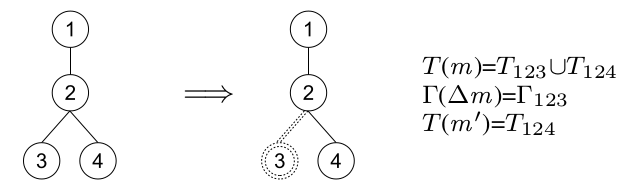
\includegraphics[width=10cm]{immagini/recert/AdattamentoCertificazione.png}
}
\caption{Adattamento della Certificazione \cite{CertEvolutiva}}\label{fig:AdattamCert}
\end{figure}


\item \textit{Ri-certificazione parziale}: al momento del rilascio di una nuova versione del servizio, inizia un nuovo processo di certificazione. In questo caso deve essere generata solo una porzione delle evidenze del certificato originale.
Questo approccio viene utilizzato al rilascio del servizio e si pone l'obiettivo di riutilizzare le evidenze esistenti per generare un nuovo certificato. Affinché ciò possa avvenire, bisogna effettuare un'analisi differenziale sul codice sorgente e del \textit{service-model} e valutare i cambiamenti \cite{CertEvolutiva}.

Ci possono essere due casistiche:
\begin{itemize}
\item Estensione, in Figura \ref{fig:PartialRecertExt}
\item Riduzione, in Figura \ref{fig:PartialRecertRed}
\end{itemize}

\begin{figure}[H]

 \begin{minipage}[b]{5.5cm}
   \centering
   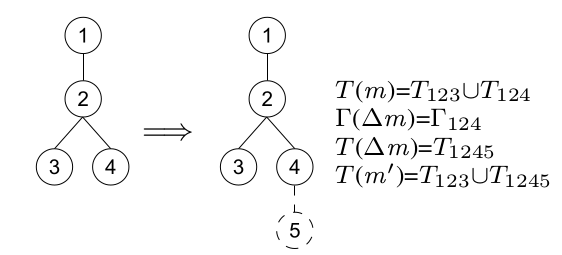
\includegraphics[width=8cm]{immagini/recert/PartialRecertExt1.png}
 \end{minipage}
 \ \hspace{2mm} \hspace{3mm} \
 \begin{minipage}[b]{5.5cm}
  \centering
   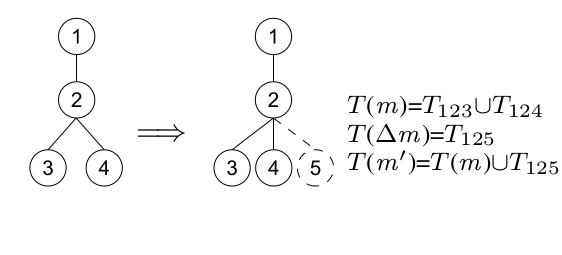
\includegraphics[width=8cm]{immagini/recert/PartialRecertExt2.png}
 \end{minipage}
    \caption{Ricertificazione parziale - Estensione \cite{CertEvolutiva}}\label{fig:PartialRecertExt}
\end{figure}

\begin{figure}[H]
 \begin{minipage}[b]{5.5cm}
   \centering
   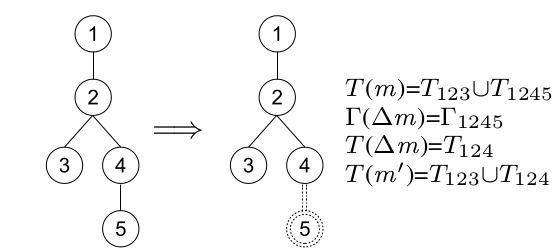
\includegraphics[width=8cm]{immagini/recert/PartialRecertRed1.png}
 \end{minipage}
 \ \hspace{2mm} \hspace{3mm} \
 \begin{minipage}[b]{5.5cm}
  \centering
   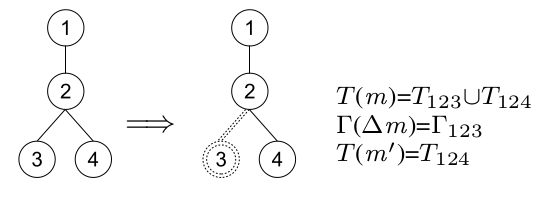
\includegraphics[width=8cm]{immagini/recert/PartialRecertRed2.png}
 \end{minipage}
    \caption{Ricertificazione parziale - Riduzione \cite{CertEvolutiva}}\label{fig:PartialRecertRed}
\end{figure}

\item \textit{Ri-certificazione totale}: al momento del rilascio di una nuova versione del servizio, inizia un nuovo processo di certificazione, senza tenere conto dei precedenti certificati emessi.
Essa viene effettuata nel momento in cui un aggiornamento del servizio effettua cambiamenti sostanziali (ad es. funzionalità orizzontali, come meccanismi di crittografia. Tutti i casi di test vengono ritenuti invalidi e il processo di certificazione viene rieffettuato dall'inizio \cite{CertEvolutiva}.
\end{itemize}

\begin{figure}[H]
   \centering
   \makebox[\textwidth]{
   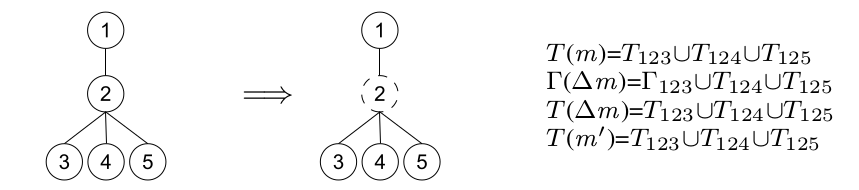
\includegraphics[width=10cm]{immagini/recert/FullRecert.png}
   }
   \caption{Ricertificazione totale \cite{CertEvolutiva}}\label{fig:FullRecert}
\end{figure}
\vfill
\newpage

%intro Viewpoint Cloud Services Certification

%sesar
%Towards the certification of cloud services
%A Certification Process for Cloud-based Services
%A Certification-Based Trust Model for Autonomic Cloud Computing Systems
%Certifying Services in Cloud- The Case for a Hybrid, Incremental and Multi-Layer Approach 

%other
%Dynamic Certification of Cloud Services
%other certificazione continuativa
%What is Really Going on at Your Cloud Service Provider? Creating Trustworthy Certifications by Continuous Auditing
%Continuous Certification of Non-Repudiation in Cloud Storage Services 

%+ paper cumulus
\end{document}